% Options for packages loaded elsewhere
\PassOptionsToPackage{unicode}{hyperref}
\PassOptionsToPackage{hyphens}{url}
%
\documentclass[
]{article}
\usepackage{lmodern}
\usepackage{amssymb,amsmath}
\usepackage{ifxetex,ifluatex}
\ifnum 0\ifxetex 1\fi\ifluatex 1\fi=0 % if pdftex
  \usepackage[T1]{fontenc}
  \usepackage[utf8]{inputenc}
  \usepackage{textcomp} % provide euro and other symbols
\else % if luatex or xetex
  \usepackage{unicode-math}
  \defaultfontfeatures{Scale=MatchLowercase}
  \defaultfontfeatures[\rmfamily]{Ligatures=TeX,Scale=1}
\fi
% Use upquote if available, for straight quotes in verbatim environments
\IfFileExists{upquote.sty}{\usepackage{upquote}}{}
\IfFileExists{microtype.sty}{% use microtype if available
  \usepackage[]{microtype}
  \UseMicrotypeSet[protrusion]{basicmath} % disable protrusion for tt fonts
}{}
\makeatletter
\@ifundefined{KOMAClassName}{% if non-KOMA class
  \IfFileExists{parskip.sty}{%
    \usepackage{parskip}
  }{% else
    \setlength{\parindent}{0pt}
    \setlength{\parskip}{6pt plus 2pt minus 1pt}}
}{% if KOMA class
  \KOMAoptions{parskip=half}}
\makeatother
\usepackage{xcolor}
\IfFileExists{xurl.sty}{\usepackage{xurl}}{} % add URL line breaks if available
\IfFileExists{bookmark.sty}{\usepackage{bookmark}}{\usepackage{hyperref}}
\hypersetup{
  pdftitle={treats: a modular R package for simulating trees and traits.},
  pdfauthor={Thomas Guillerme\^{}1},
  hidelinks,
  pdfcreator={LaTeX via pandoc}}
\urlstyle{same} % disable monospaced font for URLs
\usepackage[margin=1in]{geometry}
\usepackage{color}
\usepackage{fancyvrb}
\newcommand{\VerbBar}{|}
\newcommand{\VERB}{\Verb[commandchars=\\\{\}]}
\DefineVerbatimEnvironment{Highlighting}{Verbatim}{commandchars=\\\{\}}
% Add ',fontsize=\small' for more characters per line
\usepackage{framed}
\definecolor{shadecolor}{RGB}{248,248,248}
\newenvironment{Shaded}{\begin{snugshade}}{\end{snugshade}}
\newcommand{\AlertTok}[1]{\textcolor[rgb]{0.94,0.16,0.16}{#1}}
\newcommand{\AnnotationTok}[1]{\textcolor[rgb]{0.56,0.35,0.01}{\textbf{\textit{#1}}}}
\newcommand{\AttributeTok}[1]{\textcolor[rgb]{0.77,0.63,0.00}{#1}}
\newcommand{\BaseNTok}[1]{\textcolor[rgb]{0.00,0.00,0.81}{#1}}
\newcommand{\BuiltInTok}[1]{#1}
\newcommand{\CharTok}[1]{\textcolor[rgb]{0.31,0.60,0.02}{#1}}
\newcommand{\CommentTok}[1]{\textcolor[rgb]{0.56,0.35,0.01}{\textit{#1}}}
\newcommand{\CommentVarTok}[1]{\textcolor[rgb]{0.56,0.35,0.01}{\textbf{\textit{#1}}}}
\newcommand{\ConstantTok}[1]{\textcolor[rgb]{0.00,0.00,0.00}{#1}}
\newcommand{\ControlFlowTok}[1]{\textcolor[rgb]{0.13,0.29,0.53}{\textbf{#1}}}
\newcommand{\DataTypeTok}[1]{\textcolor[rgb]{0.13,0.29,0.53}{#1}}
\newcommand{\DecValTok}[1]{\textcolor[rgb]{0.00,0.00,0.81}{#1}}
\newcommand{\DocumentationTok}[1]{\textcolor[rgb]{0.56,0.35,0.01}{\textbf{\textit{#1}}}}
\newcommand{\ErrorTok}[1]{\textcolor[rgb]{0.64,0.00,0.00}{\textbf{#1}}}
\newcommand{\ExtensionTok}[1]{#1}
\newcommand{\FloatTok}[1]{\textcolor[rgb]{0.00,0.00,0.81}{#1}}
\newcommand{\FunctionTok}[1]{\textcolor[rgb]{0.00,0.00,0.00}{#1}}
\newcommand{\ImportTok}[1]{#1}
\newcommand{\InformationTok}[1]{\textcolor[rgb]{0.56,0.35,0.01}{\textbf{\textit{#1}}}}
\newcommand{\KeywordTok}[1]{\textcolor[rgb]{0.13,0.29,0.53}{\textbf{#1}}}
\newcommand{\NormalTok}[1]{#1}
\newcommand{\OperatorTok}[1]{\textcolor[rgb]{0.81,0.36,0.00}{\textbf{#1}}}
\newcommand{\OtherTok}[1]{\textcolor[rgb]{0.56,0.35,0.01}{#1}}
\newcommand{\PreprocessorTok}[1]{\textcolor[rgb]{0.56,0.35,0.01}{\textit{#1}}}
\newcommand{\RegionMarkerTok}[1]{#1}
\newcommand{\SpecialCharTok}[1]{\textcolor[rgb]{0.00,0.00,0.00}{#1}}
\newcommand{\SpecialStringTok}[1]{\textcolor[rgb]{0.31,0.60,0.02}{#1}}
\newcommand{\StringTok}[1]{\textcolor[rgb]{0.31,0.60,0.02}{#1}}
\newcommand{\VariableTok}[1]{\textcolor[rgb]{0.00,0.00,0.00}{#1}}
\newcommand{\VerbatimStringTok}[1]{\textcolor[rgb]{0.31,0.60,0.02}{#1}}
\newcommand{\WarningTok}[1]{\textcolor[rgb]{0.56,0.35,0.01}{\textbf{\textit{#1}}}}
\usepackage{graphicx}
\makeatletter
\def\maxwidth{\ifdim\Gin@nat@width>\linewidth\linewidth\else\Gin@nat@width\fi}
\def\maxheight{\ifdim\Gin@nat@height>\textheight\textheight\else\Gin@nat@height\fi}
\makeatother
% Scale images if necessary, so that they will not overflow the page
% margins by default, and it is still possible to overwrite the defaults
% using explicit options in \includegraphics[width, height, ...]{}
\setkeys{Gin}{width=\maxwidth,height=\maxheight,keepaspectratio}
% Set default figure placement to htbp
\makeatletter
\def\fps@figure{htbp}
\makeatother
\setlength{\emergencystretch}{3em} % prevent overfull lines
\providecommand{\tightlist}{%
  \setlength{\itemsep}{0pt}\setlength{\parskip}{0pt}}
\setcounter{secnumdepth}{-\maxdimen} % remove section numbering
\newlength{\cslhangindent}
\setlength{\cslhangindent}{1.5em}
\newenvironment{cslreferences}%
  {\setlength{\parindent}{0pt}%
  \everypar{\setlength{\hangindent}{\cslhangindent}}\ignorespaces}%
  {\par}

\title{\texttt{treats}: a modular \texttt{R} package for simulating
trees and traits.}
\author{Thomas Guillerme\(^1\)}
\date{2023-06-07}

\begin{document}
\maketitle

\(^1\) School of Biosciences, University of Sheffield, Sheffield, S10
2TN, United Kingdom.
\href{mailto:guillert@tcd.ie}{\nolinkurl{guillert@tcd.ie}}

Running head: \texttt{treats}: TREes And Traits Simulations

\hypertarget{abstract}{%
\section{Abstract}\label{abstract}}

\begin{enumerate}
\def\labelenumi{\arabic{enumi}.}
\item
  Simulating biological realistic data is an important step to
  understand and investigate biodiversity. Simulated data can be used to
  generate null, base line or neutral models. These can be used either
  in comparison to observed data to estimate the mechanisms that
  generated the data. Or they can be used to explore, understand and
  develop theoretical advances by proposing toy models.
\item
  In evolutionary biology, simulations often involve the need of an
  evolutionary process where descent with modification is at the core of
  how the simulated data is generated. These evolutionary processes can
  then be nearly infinitely modified to include complex processes that
  affect the simulations such as traits co-evolution, competition
  mechanisms or mass extinction events.
\item
  Here I present the \texttt{treats} package, a modular \texttt{R}
  package for trees and traits simulations. This package is based on a
  simple birth death algorithm from which all steps can easily be
  modified by users. It also provides a tidy interface through the
  \texttt{treats} object, allowing users to easily run reproducible
  simulations. It also comes with an extend manual regularly updated
  following users' questions or suggestions.
\end{enumerate}

Keywords: trees, traits, simulations, birth-death, null-models, ecology,
evolution, disparity

\hypertarget{introduction}{%
\section{Introduction}\label{introduction}}

Comparing biological patterns is one of the key ways to understand
mechanisms in evolutionary biology. This lead to the development of
phylogenetic comparative methods as key methodologically driven topic in
ecology, evolution and palaeontology (Felsenstein 1985; Pennell and
Harmon 2013). As indicated in the name, phylogenetic comparative methods
rely on comparing patterns in a phylogenetic context to understand
biological mechanisms or concepts (Harmon 2019). These comparisons can
be done between observed patterns under different conditions or against
null, neutral or baseline models (see Bausman (2018) for distinctions)
suggesting different processes or mechanisms. For example different
traits distribution for species with different diets (Deepak, Gower, and
Cooper 2023), or habitats (Pinto-Ledezma et al. 2017) or by comparing
some observed pattern to one simulated under null or base conditions
(Miller et al. 2022). In theory, workers can follow the research
pipeline of thinking of a specific mechanism (e.g.~mass extinction
allowing the surviving species to acquire new morphologies), collect
some data to test this mechanism (e.g.~some traits of species across and
extinction event) and then compare these patterns to one simulated under
no specific conditions (e.g.~a null model where the traits evolve
randomly regardless of an extinction event Puttick, Guillerme, and Wills
(2020)). For such an approach, we need statistical and softwares
solutions to simulate trees and data to generate these specific null
models.

In practice, these evolutionary simulations can be done relatively
easily on computers using a birth-death process (Feller 1939; Stadler
2010; FitzJohn 2012). A birth-death process is a continuous time Markov
process that had been routinely implemented in \texttt{R} (R Core Team
2023) to simulate biological phylogenies (e.g.~(Paradis and Schliep
2019), (FitzJohn 2012)). These algorithm to generate phylogenetic trees
can be coupled with other Markov processes to also generate traits, for
example using a Brownian Motion process (BM; Cavalli-Sforza and Edwards
(1967)) or an Ornstein Uhlenbeck (OU; Lande (1976); see Cooper et al.
(2016) for a distinction between both). In \texttt{R}, this can be done
with several already well used and well documented packages. For example
if you want to simulate diversity through time, you can use
\texttt{TreeSim} (Stadler 2011) to simulate diversity under a set of
specific parameters (e.g.~speciation and extinction) with some events
disrupting the simulations (e.g.~mass extinctions). One can even improve
on generating these patterns using \texttt{FossilSim} (Barido-Sottani et
al. 2019) to generate a pattern that will take into account
fossilization processes. Or use \texttt{paleobuddy} (Rosario Petrucci,
Januario, and Quental 2022) or \texttt{paleotree} (Bapst 2012) to
generate palaeontology specific data. On the other hand, if you need to
simulate both diversity and traits through time, this can be done with
specific parameters in \texttt{RPANDA} (Morlon et al. 2016) or in
\texttt{PETER} (Puttick, Guillerme, and Wills 2020) where the traits are
generated stochasticaly through time (given some process) during the
birth-death process.

Although the packages mentioned above are excellent and routinely used
with fast and reliable algorithms and associated documentation, they are
all designed for specific tasks and don't allow much modification beyond
the input parameters designed by the authors. For example,
\texttt{TreeSim} can simulate a birth-death tree with some extinction
event but is not designed to simulated one with an extinction event that
leads to the birth-death process to be not diversity dependent anymore
(e.g.~simulating a release in selection pressure after the extinction
process that leads to a different process dominating speciation). Or
\texttt{PETER} is not designed to simulate a complex set of traits (say
three correlated BM traits and two independent OU ones). This absence of
modularity has hampered the use of complex and question tailored
simulations evolutionary biology, although I acknowledge this was not
the primary aim of the authors of the packages mentioned above. This has
led workers to often develop their own tools to answer specific
questions (e.g.~Puttick, Guillerme, and Wills (2020)). Therefore, we
propose \texttt{treats} a modular \texttt{R} package to simulate both
diversity and disparity through time.

\hypertarget{description}{%
\section{Description}\label{description}}

\texttt{treats} is based on the eponymous \texttt{treats} function that
allows to simulate a phylogeny and some trait(s) simultaneously. The
base birth-death algorithm ``grows'' a phylogenetic tree and generates
traits for each node and tips in the following manner:

\begin{enumerate}
\def\labelenumi{\arabic{enumi}.}
\tightlist
\item
  Generating branch length;
\item
  Selecting a lineage among the currently living ones;
\item
  Choosing whether that lineage goes extinct (becomes a tip) or
  speciates (becomes a node).
\end{enumerate}

These four steps are repeated until the tree reaches the desired age or
number of species. If traits are simulated during the process, a fourth
step is added:

\begin{enumerate}
\def\labelenumi{\arabic{enumi}.}
\setcounter{enumi}{3}
\tightlist
\item
  Generating some trait(s) value(s) for the selected lineage (no either
  a tip or a node).
\end{enumerate}

In \texttt{treats}, these three or four steps are implemented as modular
functions that the user can easily change using an internal class of
objects called \texttt{"modifiers"} or \texttt{"traits"} (Fig.
\ref{Fig:workflow}). The simulation then outputs a tree (of class
\texttt{"phylo"} and a associated table of traits - \texttt{"matrix"})
that can be visualised using the \texttt{plot.treats} function. A third
class of object called \texttt{"events"} can be added to the simulations
to modify it under certain conditions (e.g.~simulating a mass
extinction). Each element in the algorithm described above can be
modified by the user using the implemented functions
\texttt{make.bd.params} to set the birth-death parameters,
\texttt{make.traits} to set the trait(s), \texttt{make.modifiers} to set
the birth-death algorithm and \texttt{make.events} to eventually add one
or more events.

\begin{figure}
\hypertarget{figure1}{%
\centering
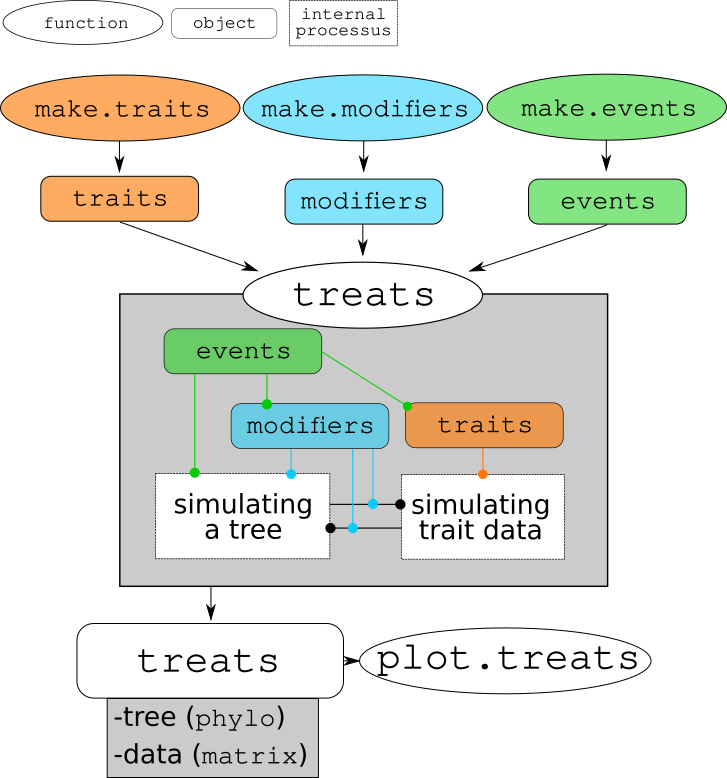
\includegraphics{../inst/gitbook/treats_structure.png}
\caption{Figure 1: \texttt{treats} package workflow: the \texttt{treats}
algorithm generates a tree and traits using inbuilt \texttt{"traits"}
objects that contain the instructions on how to generate the trait data
(e.g.~which process? how many dimensions?); \texttt{"modifiers"} objects
that contains instructions on how to ``grow'' the tree (e.g.~by linking
speciation to trait values, or to the current number of species); and
\texttt{"events"} objects that can modify the tree structure,
\texttt{"modifiers"} or \texttt{"traits"} depending on specific
conditions (e.g.~80\% of species with positive trait values go extinct
after reaching a specific time).}\label{figure1}
}
\end{figure}

\hypertarget{brief-applied-example}{%
\subsection{Brief applied example}\label{brief-applied-example}}

The modularity structure of the \texttt{treats} packages allows users to
design complex simulation scenarios to fit their specific question and
data. To illustrate this we will look whether it is possible to detect
changes in disparity (i.e.~diversity of traits) in a subset of the data
published from Beck and Lee (2014) implemented in Guillerme (2018). This
dataset contains the ordinated traits for 50 mammalian species across
the cretaceous-palaeogene extinction event (K-Pg, 66 Mya; Fig. 2).

\begin{Shaded}
\begin{Highlighting}[]
\CommentTok{\#\# Loading the data and packages}
\KeywordTok{library}\NormalTok{(treats)}
\KeywordTok{library}\NormalTok{(dispRity)}
\KeywordTok{data}\NormalTok{(BeckLee\_tree)}
\KeywordTok{data}\NormalTok{(BeckLee\_mat99)}

\CommentTok{\#\# Creating the time slices}
\NormalTok{time\_slices \textless{}{-}}\StringTok{ }\KeywordTok{chrono.subsets}\NormalTok{(BeckLee\_mat99, BeckLee\_tree,}
                              \DataTypeTok{method =} \StringTok{"continuous"}\NormalTok{,}
                              \DataTypeTok{model  =} \StringTok{"acctran"}\NormalTok{,}
                              \DataTypeTok{time   =} \KeywordTok{seq}\NormalTok{(}\DataTypeTok{from =} \DecValTok{96}\NormalTok{, }\DataTypeTok{to =} \DecValTok{36}\NormalTok{, }\DataTypeTok{by =} \DecValTok{{-}10}\NormalTok{))}

\CommentTok{\#\# Calculating disparity on the two first dimensions only}
\NormalTok{observed\_disparity \textless{}{-}}\StringTok{ }\KeywordTok{dispRity}\NormalTok{(}\KeywordTok{boot.matrix}\NormalTok{(time\_slices),}
                               \DataTypeTok{metric =} \KeywordTok{c}\NormalTok{(sum, variances),}
                               \DataTypeTok{dimensions =} \KeywordTok{c}\NormalTok{(}\DecValTok{1}\NormalTok{,}\DecValTok{2}\NormalTok{))}
\end{Highlighting}
\end{Shaded}

\begin{figure}
\centering
\includegraphics{treats_paper_files/figure-latex/prepdata-1.pdf}
\caption{Figure 2: Observed phylogeny (A) and disparity through time (B)
in the subset of Beck and Lee (2014)'s dataset. For this specific data,
is it possible to detect potential changes of disparity due to a mass
extinction event?}
\end{figure}

Using this example dataset, one might be interested in testing whether
the K-Pg extinction had an effect on disparity through time. But can
such effect be detected in the first place? We can test this by
simulating some datasets with similar properties as the observed data
and measure changes in disparity in these simulated datasets.

\hypertarget{simulating-trees}{%
\subsubsection{Simulating trees}\label{simulating-trees}}

The first and simplest way is to simulate tree topologies that have
similar properties than the observed one. To do so, we need to use some
\textbf{speciation} parameter indicating the rate at which lineages
speciate (\emph{aka} ``birth'' or ``\(\lambda\)'') and an
\textbf{extinction} parameter indicating the rate at which they go
extinct (\emph{aka} ``death'' or ``\(\mu\)''). These two parameters can
be crudely calculated from a give tree by counting the number of
speciations and extinctions through time (but see better methods,
e.g.~\texttt{ape::birthdeath}; Lawton, May, and Raup (1995); Paradis and
Schliep (2019)). We also need a stopping rule for when to stop the
simulations (in our case when reaching 30 time units). This will produce
a single random tree using the input parameters (Fig. 3). Note that I
will not discuss the options here in great details. Much more
information can be found in the
\href{http://tguillerme.github.io/treats.html}{\texttt{treats} manual}.

\begin{Shaded}
\begin{Highlighting}[]
\CommentTok{\#\# Using the birth{-}death parameters from the observed tree}
\NormalTok{my\_bd\_params \textless{}{-}}\StringTok{ }\KeywordTok{crude.bd.est}\NormalTok{(BeckLee\_tree)}
\CommentTok{\#\# Setting the stopping rule (stop after 30 time units)}
\NormalTok{stop\_rule \textless{}{-}}\StringTok{ }\KeywordTok{list}\NormalTok{(}\DataTypeTok{max.time =} \DecValTok{30}\NormalTok{)}

\CommentTok{\#\# Simulate the tree}
\KeywordTok{set.seed}\NormalTok{(}\DecValTok{1}\NormalTok{)}
\NormalTok{sim\_tree \textless{}{-}}\StringTok{ }\KeywordTok{treats}\NormalTok{(}\DataTypeTok{bd.params  =}\NormalTok{ my\_bd\_params,}
                   \DataTypeTok{stop.rule  =}\NormalTok{ stop\_rule,}
                   \DataTypeTok{null.error =} \DecValTok{100}\NormalTok{)}
\end{Highlighting}
\end{Shaded}

\begin{figure}
\centering
\includegraphics{treats_paper_files/figure-latex/simtree-1.pdf}
\caption{Figure 3: A randomly simulated tree with similar properties as
the observed one. Note that the time here is expressed in arbitrary
units.}
\end{figure}

\hypertarget{simulating-trees-and-traits}{%
\subsubsection{Simulating trees and
traits}\label{simulating-trees-and-traits}}

For our specific question, we will also need to simulate some traits
associated with each node and tip. For simplicity we will simulate a two
dimensional Brownian Motion trait. To do so, we can create a
\texttt{"traits"} object with the function \texttt{make.traits}. This
results in a 2 dimensional trait space for all the simulated species and
their nodes (Fig. 4).

\begin{Shaded}
\begin{Highlighting}[]
\CommentTok{\#\# Creating a trait in 2 dimensions.}
\NormalTok{my\_traits \textless{}{-}}\StringTok{ }\KeywordTok{make.traits}\NormalTok{(}\DataTypeTok{process =}\NormalTok{ BM.process, }\DataTypeTok{n =} \DecValTok{2}\NormalTok{)}

\CommentTok{\#\# Simulate the tree and traits}
\KeywordTok{set.seed}\NormalTok{(}\DecValTok{1}\NormalTok{)}
\NormalTok{sim\_data \textless{}{-}}\StringTok{ }\KeywordTok{treats}\NormalTok{(}\DataTypeTok{traits     =}\NormalTok{ my\_traits,}
                   \DataTypeTok{bd.params  =}\NormalTok{ my\_bd\_params,}
                   \DataTypeTok{stop.rule  =}\NormalTok{ stop\_rule,}
                   \DataTypeTok{null.error =} \DecValTok{100}\NormalTok{)}
\end{Highlighting}
\end{Shaded}

\begin{figure}
\centering
\includegraphics{treats_paper_files/figure-latex/simtreetraits-1.pdf}
\caption{Figure 4: A randomly simulated tree with a 2 dimensional random
Brownian Motion trait. Orange, light blue and dark blue dots
respectively represent nodes, fossils and living species.}
\end{figure}

\hypertarget{simulating-a-trees-and-traits-with-events}{%
\subsubsection{Simulating a trees and traits with
events}\label{simulating-a-trees-and-traits-with-events}}

To answer our question, we also want to simulate an extinction event. To
do so, we can create two different \texttt{"events"} object with the
function \texttt{make.events}. The first one will simulate a random
extinction event after reaching half of the simulations (15 time units)
and then making three quarter (0.75) of the taxa go extinct. The second
one will simulate a random extinction but based on trait values: after
reaching time 20, all the species with positive trait values will go
extinct. Both scenarios thus illustrate two different types of mass
extinction (selective and random Puttick, Guillerme, and Wills (2020)).

\begin{Shaded}
\begin{Highlighting}[]
\CommentTok{\#\# Creating a random mass extinction}
\NormalTok{random\_extinction \textless{}{-}}\StringTok{ }\KeywordTok{make.events}\NormalTok{(}
    \DataTypeTok{target       =} \StringTok{"taxa"}\NormalTok{,}
    \DataTypeTok{condition    =} \KeywordTok{time.condition}\NormalTok{(}\DecValTok{15}\NormalTok{),}
    \DataTypeTok{modification =} \KeywordTok{random.extinction}\NormalTok{(}\FloatTok{0.75}\NormalTok{))}
\CommentTok{\#\# Creating an extinction that removes species with positive trait values}
\NormalTok{positive\_extinction \textless{}{-}}\StringTok{ }\KeywordTok{make.events}\NormalTok{(}
    \DataTypeTok{target =} \StringTok{"taxa"}\NormalTok{,}
    \DataTypeTok{condition =} \KeywordTok{time.condition}\NormalTok{(}\DecValTok{15}\NormalTok{),}
    \DataTypeTok{modification =} \KeywordTok{trait.extinction}\NormalTok{(}\DataTypeTok{x =} \DecValTok{0}\NormalTok{, }\DataTypeTok{condition =} \StringTok{\textasciigrave{}}\DataTypeTok{\textgreater{}=}\StringTok{\textasciigrave{}}\NormalTok{))}

\KeywordTok{set.seed}\NormalTok{(}\DecValTok{2}\NormalTok{)}
\CommentTok{\#\# Simulate the tree and traits with a random extinction event}
\NormalTok{sim\_rand\_extinction \textless{}{-}}\StringTok{ }\KeywordTok{treats}\NormalTok{(}
                   \DataTypeTok{traits     =}\NormalTok{ my\_traits,}
                   \DataTypeTok{bd.params  =}\NormalTok{ my\_bd\_params,}
                   \DataTypeTok{stop.rule  =}\NormalTok{ stop\_rule,}
                   \DataTypeTok{events     =}\NormalTok{ random\_extinction,}
                   \DataTypeTok{null.error =} \DecValTok{100}\NormalTok{,}
                   \DataTypeTok{replicates =} \DecValTok{50}\NormalTok{)}

\CommentTok{\#\# Simulate the tree and traits with a random extinction event}
\NormalTok{sim\_trait\_extinction \textless{}{-}}\StringTok{ }\KeywordTok{treats}\NormalTok{(}
                   \DataTypeTok{traits     =}\NormalTok{ my\_traits,}
                   \DataTypeTok{bd.params  =}\NormalTok{ my\_bd\_params,}
                   \DataTypeTok{stop.rule  =}\NormalTok{ stop\_rule,}
                   \DataTypeTok{events     =}\NormalTok{ positive\_extinction,}
                   \DataTypeTok{null.error =} \DecValTok{100}\NormalTok{,}
                   \DataTypeTok{replicates =} \DecValTok{50}\NormalTok{)}
\end{Highlighting}
\end{Shaded}

\begin{figure}
\centering
\includegraphics{treats_paper_files/figure-latex/simtreetraitsevents-1.pdf}
\caption{Figure 5: Two different mass extinction events: (A) 75\% of
species go extinct; (B) all species with positive trait values go
extinct. The red line marks the extinction event.}
\end{figure}

Once we have simulated a distribution of trees and traits with the two
extinction scenarios, we can measure disparity as in Fig. 1 for all the
simulated data and compare it to the observed disparity.

\begin{figure}
\centering
\includegraphics{treats_paper_files/figure-latex/simdisparity-1.pdf}
\caption{Figure 6: Comparison of the observed sum of variances (dashed
line) to the simulated one (ligth and dark grey polygons and black line
representing respectively the 95\% and 50\% confidence interval and the
median value).}
\end{figure}

From these results we can draw some preliminary conclusions: the
observed change in disparity is more likely due to a random mass
extinction rather than a selective one. This is of course a crude way of
testing this, a more rigorous approach is likely needed to answer the
question (i.e.~more and better quality data, and more thorough methods,
e.g.~using a rank envelope test Murrell (2018)).

\hypertarget{major-functionalities}{%
\subsection{Major functionalities}\label{major-functionalities}}

The following sections provide an overview of the three main functions
displayed in Figure 1 (\texttt{make.traits}, \texttt{make.modifiers} and
\texttt{make.events}).

\hypertarget{simulating-traits}{%
\subsubsection{Simulating traits}\label{simulating-traits}}

Traits are simulated via the \texttt{make.traits} function given one or
more processes, number of dimensions per process and some starting
value(s). Essentially, the generation of new trait values is based on a
process (a \texttt{function}) modifying a trait value (\texttt{x0})
relative to some branch length (\texttt{edge.length}). For example, a
simple Brownian Motion process could be generated by the function
\texttt{rnorm} where the it modifies the trait value \texttt{x0}
relative to the branch length (\texttt{edge.length}). The longer the
branch length, the more likely the new trait value will be different
from \texttt{x0}:

\begin{Shaded}
\begin{Highlighting}[]
\CommentTok{\#\# Functionalising the previous example of a Brownian Motion process}
\NormalTok{my.bm.process \textless{}{-}}\StringTok{ }\ControlFlowTok{function}\NormalTok{(x0, edge.length) \{}
    \KeywordTok{rnorm}\NormalTok{(}\DataTypeTok{n =} \DecValTok{1}\NormalTok{, }\DataTypeTok{mean =}\NormalTok{ x0, }\DataTypeTok{sd =}\NormalTok{ edge.length)}
\NormalTok{\} }
\CommentTok{\#\# Creating the traits object}
\NormalTok{my.trait \textless{}{-}}\StringTok{ }\KeywordTok{make.traits}\NormalTok{(}\DataTypeTok{process =}\NormalTok{ my.bm.process)}
\end{Highlighting}
\end{Shaded}

Of course biological data can be much more complex and often
multivariate (Adams and Collyer 2019) requiring the users to develop
more complex function to cater their specific needs. However, the
\texttt{treats} package contains a list of pre-built processes that are
``ready-to-use'':

\begin{itemize}
\tightlist
\item
  \texttt{BM.process} and \texttt{OU.process}: generalised Brownian
  Motion and Ornstein-Uhlenbeck processes in any number of dimensions
  (including possible correlation);
\item
  \texttt{multi.peak.process}: a generalised Ornstein-Uhlenbeck process
  (uni- or multi-dimensional) which allows for multiple peaks (usually
  called the ``alpha'' parameters; Lande (1976));
\item
  \texttt{repulsion.process}: a unidimensional process generating trait
  values that don't overlap with previously generated trait values;
\item
  \texttt{discrete.process}: generates discrete trait values;
\item
  \texttt{no.process}: ignores the branch length (i.e.~a time
  independent process);
\end{itemize}

Note that the \texttt{treats} package primary aim is to generate both a
tree and some traits at the same time. However, it is possible to also
just generate traits with a given topology. This is done through the
function \texttt{map.traits} that intakes one or more trees and a
\texttt{"traits"} object.

\hypertarget{modifying-the-birth-death-process}{%
\subsubsection{Modifying the birth-death
process}\label{modifying-the-birth-death-process}}

Modifying the birth-death process can be done in several ways. Most
easily it is done through changing the stopping rules through the
\texttt{stop.rule} argument (number of total taxa or living ones, or
time of the simulation). Equally straightforward, one can modify the
parameters of the birth-death process through the
\texttt{make.bd.params} function: the speciation (\(\lambda\)) and the
extinction (\(\mu\)) ones. These can be either fixed values (for
constant speciation and extinction) or values drawn from distributions.

It is also possible to directly modify how the birth-death algorithm
works through \texttt{make.modifiers} by changing the three main
components of the birth-death algorithm as described above. By default,
the algorithm uses the following algorithms:

\begin{enumerate}
\def\labelenumi{\arabic{enumi}.}
\tightlist
\item
  \textbf{Generating branch length} by drawing a value from an
  exponential distribution with the rate being function of the current
  number of lineages scaled by the speciation and extinction parameters
\end{enumerate}

\begin{Shaded}
\begin{Highlighting}[]
\CommentTok{\#\# The default branch length generation}
\KeywordTok{rexp}\NormalTok{(}\DecValTok{1}\NormalTok{, }\DataTypeTok{rate =}\NormalTok{ number\_of\_lineages }\OperatorTok{*}\StringTok{ }\NormalTok{(speciation }\OperatorTok{+}\StringTok{ }\NormalTok{extinction))}
\end{Highlighting}
\end{Shaded}

\begin{enumerate}
\def\labelenumi{\arabic{enumi}.}
\setcounter{enumi}{1}
\tightlist
\item
  \textbf{Selecting a lineage} among the currently living ones by simply
  sampling across the available (living) lineages:
\end{enumerate}

\begin{Shaded}
\begin{Highlighting}[]
\CommentTok{\#\# The default lineage selection}
\KeywordTok{sample}\NormalTok{(number\_of\_lineages, }\DecValTok{1}\NormalTok{)}
\end{Highlighting}
\end{Shaded}

\begin{enumerate}
\def\labelenumi{\arabic{enumi}.}
\setcounter{enumi}{2}
\tightlist
\item
  C\textbf{hoosing whether that lineage goes extinct (becomes a tip) or
  speciates (becomes a node)} by drawing a random number between 0 and 1
  and comparing it to the ratio of speciation and turnover (speciation +
  extinction). If the random number is smaller than the ratio of
  speciation and turnover, the lineage speciates, else it goes extinct:
\end{enumerate}

\begin{Shaded}
\begin{Highlighting}[]
\CommentTok{\#\# The default speciation/extinction decider}
\KeywordTok{runif}\NormalTok{(}\DecValTok{1}\NormalTok{) }\OperatorTok{\textless{}=}\StringTok{ }\NormalTok{(speciation }\OperatorTok{/}\StringTok{ }\NormalTok{(speciation }\OperatorTok{+}\StringTok{ }\NormalTok{extinction))}
\end{Highlighting}
\end{Shaded}

The function \texttt{make.modifiers} allows to specifically change any
of these components by providing a different function for each part of
the algorithm. For example, we could modify the three functions above so
that the branch length is not dependent on the number of lineages, the
sampling is always the first species available and the extinction is
drawn from a normal distribution. Note that these function need a
specific syntax that is detailed in the
\href{http://tguillerme.github.io/treats.html}{\texttt{treats} manual}.

\begin{Shaded}
\begin{Highlighting}[]
\CommentTok{\#\# Lineage independent waiting:}
\NormalTok{lineage.independent \textless{}{-}}\StringTok{ }\ControlFlowTok{function}\NormalTok{(bd.params,}
                                \DataTypeTok{lineage =} \OtherTok{NULL}\NormalTok{,}
                                \DataTypeTok{trait.values =} \OtherTok{NULL}\NormalTok{,}
                                \DataTypeTok{modify.fun =} \OtherTok{NULL}\NormalTok{) \{}
\NormalTok{    my\_rate \textless{}{-}}\StringTok{ }\NormalTok{bd.params}\OperatorTok{$}\NormalTok{speciation }\OperatorTok{+}\StringTok{ }\NormalTok{bd.params}\OperatorTok{$}\NormalTok{extinction}
    \KeywordTok{return}\NormalTok{(}\KeywordTok{rexp}\NormalTok{(}\DecValTok{1}\NormalTok{, }\DataTypeTok{rate =}\NormalTok{ my\_rate))}
\NormalTok{\}}
\CommentTok{\#\# Selecting always the first species}
\NormalTok{select.first \textless{}{-}}\StringTok{ }\ControlFlowTok{function}\NormalTok{(bd.params,}
                         \DataTypeTok{lineage =} \OtherTok{NULL}\NormalTok{,}
                         \DataTypeTok{trait.values =} \OtherTok{NULL}\NormalTok{,}
                         \DataTypeTok{modify.fun =} \OtherTok{NULL}\NormalTok{) \{}
    \KeywordTok{return}\NormalTok{(}\KeywordTok{as.integer}\NormalTok{(}\DecValTok{1}\NormalTok{))}
\NormalTok{\}}
\CommentTok{\#\# Random normal speciation}
\NormalTok{normal.speciation \textless{}{-}}\StringTok{ }\ControlFlowTok{function}\NormalTok{(bd.params,}
                              \DataTypeTok{lineage =} \OtherTok{NULL}\NormalTok{,}
                              \DataTypeTok{trait.values =} \OtherTok{NULL}\NormalTok{,}
                              \DataTypeTok{modify.fun =} \OtherTok{NULL}\NormalTok{) \{}
\NormalTok{    my\_turnover \textless{}{-}}\StringTok{ }\NormalTok{bd.params}\OperatorTok{$}\NormalTok{speciation}\OperatorTok{/}
\StringTok{                  }\NormalTok{(bd.params}\OperatorTok{$}\NormalTok{speciation }\OperatorTok{+}\StringTok{ }\NormalTok{bd.params}\OperatorTok{$}\NormalTok{extinction)}
    \KeywordTok{return}\NormalTok{(}\KeywordTok{rnorm}\NormalTok{(}\DecValTok{1}\NormalTok{) }\OperatorTok{\textless{}=}\StringTok{ }\NormalTok{my\_turnover)}
\NormalTok{\}}

\CommentTok{\#\# Creating the modifier object}
\NormalTok{modified.birth.death \textless{}{-}}\StringTok{ }\KeywordTok{make.modifiers}\NormalTok{(}\DataTypeTok{branch.length =}\NormalTok{ lineage.independent,}
                                       \DataTypeTok{selection     =}\NormalTok{ select.first,}
                                       \DataTypeTok{speciation    =}\NormalTok{ normal.speciation)}
\end{Highlighting}
\end{Shaded}

\hypertarget{creating-events}{%
\subsubsection{Creating events}\label{creating-events}}

The final major argument to be passed to \texttt{treats} are the
\texttt{"events"} objects generated through \texttt{make.events} where
the following information needs to be specified:

\begin{itemize}
\tightlist
\item
  the \texttt{target} designating what the event should be applied to
  (e.g.~\texttt{"taxa"} for modifying the number of species,
  \texttt{"traits"} for modifying the traits, etc.)
\item
  the \texttt{condition} which is a function returning a logical value
  of when to trigger the event (e.g.~when reaching a certain number of
  taxa, after some specific time has ellapsed or if some specific trait
  value is reached, etc.)
\item
  the \texttt{modification} which is a function that specifically
  modifies an internal object in the \texttt{treats} algorithm.
\end{itemize}

For a more exhaustive list of events so you can refer to the
\href{http://tguillerme.github.io/treats.html}{\texttt{treats} manual}
with many different detailed examples. Briefly though, this is how the
mass extinction events are designed in the example above.

\begin{Shaded}
\begin{Highlighting}[]
\CommentTok{\#\# Creating an extinction that removes species with positive trait values}
\NormalTok{positive\_extinction \textless{}{-}}\StringTok{ }\KeywordTok{make.events}\NormalTok{(}
    \DataTypeTok{target       =} \StringTok{"taxa"}\NormalTok{,}
    \DataTypeTok{condition    =} \KeywordTok{time.condition}\NormalTok{(}\DecValTok{15}\NormalTok{),}
    \DataTypeTok{modification =} \KeywordTok{random.extinction}\NormalTok{(}\FloatTok{0.75}\NormalTok{))}
\end{Highlighting}
\end{Shaded}

For this event, the target is the number of taxa in the simulations.
This is indicated using the \texttt{target\ =\ "taxa"} argument. Then
the event is triggered using the argument \texttt{time.condition(15)}
and modifies the internal \texttt{lineage} object using the
\texttt{trait.extinction(x\ =\ 0,\ condition\ =\ \textasciigrave{}\textgreater{}=\textasciigrave{})}
function. \texttt{time.condition} and \texttt{trait.extinction} are both
function factories which are not gonna be detailed here (see Wickham
(2019)). Effectively these arguments can be passed directly as standard
functions. For example, to trigger the event when reaching time 15 we
can use the following function:

\begin{Shaded}
\begin{Highlighting}[]
\CommentTok{\#\# Returns TRUE when reaching time 15}
\NormalTok{reaching.time15 \textless{}{-}}\StringTok{ }\ControlFlowTok{function}\NormalTok{(bd.params, lineage, trait.values, time) \{}
    \KeywordTok{return}\NormalTok{(time }\OperatorTok{\textgreater{}}\StringTok{ }\DecValTok{15}\NormalTok{)}
\NormalTok{\}}
\end{Highlighting}
\end{Shaded}

This will trigger the \texttt{modification} which is equivalent to the
following function modifying the \texttt{lineage} internal list:

\begin{Shaded}
\begin{Highlighting}[]
\NormalTok{removing.}\FloatTok{75.}\NormalTok{taxa \textless{}{-}}\StringTok{ }\ControlFlowTok{function}\NormalTok{(bd.params, lineage, trait.values) \{}
    \CommentTok{\#\# Select a portion of the living species to go extinct}
\NormalTok{    extinct \textless{}{-}}\StringTok{ }\KeywordTok{sample}\NormalTok{(lineage}\OperatorTok{$}\NormalTok{n, }\KeywordTok{round}\NormalTok{(lineage}\OperatorTok{$}\NormalTok{n }\OperatorTok{*}\StringTok{ }\FloatTok{0.75}\NormalTok{))}

    \CommentTok{\#\# Update the lineage object}
\NormalTok{    lineage}\OperatorTok{$}\NormalTok{livings \textless{}{-}}\StringTok{ }\NormalTok{lineage}\OperatorTok{$}\NormalTok{livings[}\OperatorTok{{-}}\NormalTok{extinct]}
\NormalTok{    lineage}\OperatorTok{$}\NormalTok{n       \textless{}{-}}\StringTok{ }\NormalTok{lineage}\OperatorTok{$}\NormalTok{n }\OperatorTok{{-}}\StringTok{ }\KeywordTok{length}\NormalTok{(extinct)}
    \KeywordTok{return}\NormalTok{(lineage)}
\NormalTok{\}}
\end{Highlighting}
\end{Shaded}

Hence, the extinction event described above is equivalent to the
following one:

\begin{Shaded}
\begin{Highlighting}[]
\CommentTok{\#\# Creating an extinction that removes species with positive trait values}
\NormalTok{positive\_extinction \textless{}{-}}\StringTok{ }\KeywordTok{make.events}\NormalTok{(}
    \DataTypeTok{target       =} \StringTok{"taxa"}\NormalTok{,}
    \DataTypeTok{condition    =}\NormalTok{ reaching.time15,}
    \DataTypeTok{modification =}\NormalTok{ removing.}\FloatTok{75.}\NormalTok{taxa)}
\end{Highlighting}
\end{Shaded}

\hypertarget{visualising-results}{%
\subsubsection{Visualising results}\label{visualising-results}}

The \texttt{treats} package also comes with tools to visualise trees and
traits together or separately. This can be done through the generic S3
\texttt{plot} function (calling \texttt{plot.treats}) and allows to
display up to three traits or two traits and time (in 3D) as displayed
in Figures 4 and 5. These functions can also be used to visualise trees
and traits together from non \texttt{"treats"} objects by using the
\texttt{make.treats} function to transform them into \texttt{"treats"}
objects.

\hypertarget{additional-information}{%
\section{Additional information}\label{additional-information}}

\hypertarget{manuals-and-vignette}{%
\subsection{Manuals and vignette}\label{manuals-and-vignette}}

The \texttt{treats} package comes with internal documentation
(e.g.~\texttt{?treats}) but also with a thorough and extended vignette
in a gitbook format: the
\href{http://tguillerme.github.io/treats.html}{\texttt{treats} manual}.
This manual is designed so that it can be regularly updated and enhanced
through the lifetime of the package facilitating the interface between
methods development and usage (Cooper, Thomas, and FitzJohn 2016).

\hypertarget{further-directions}{%
\subsection{Further directions}\label{further-directions}}

This paper describes the first version of the \texttt{treats} package.
However, I intend, either personally or through collaborations to
continuously develop this package. For example future planned versions
will include: lineage specific simulations; abiotic events; time
dependent simulations and; a better integration with the
\texttt{dispRity} package. This will be done while keeping track change
(through \texttt{NEWS} file), continuous integration and unit testing.
Furthermore, I am planning to develop the GitHub page associated with
the package to encourage users to share their simulation templates and
build library from them to facilitate the work for future users.

\hypertarget{repeatability-and-reproducibility}{%
\subsection{Repeatability and
reproducibility}\label{repeatability-and-reproducibility}}

This paper is entirely reproducible from an Rmarkdown document available
on \href{https://github.com/TGuillerme/treats/paper/}{GitHub}. The data
used for the example above (Beck and Lee 2014) is available from the
\texttt{dispRity} package (Guillerme 2018).

\hypertarget{conclusion}{%
\section{Conclusion}\label{conclusion}}

The \texttt{treats} package modular architecture allows workers to
develop their own specific biological simulation scenarios based on
their own specific research question. The pipeline of the package
through the different \texttt{"treats"} objects (\texttt{"traits"},
\texttt{"modifiers"} and \texttt{"events"}) also allows workers to
generate publication standard results through plotting but also with
easily reproducible and reusable scripts.

\hypertarget{package-location}{%
\subsection{Package location}\label{package-location}}

The \texttt{treats} package is available on
\href{https://github.com/TGuillerme/treats}{GitHub} with more associated
information. All the versions of the package are archived on ZENODO with
associated
\href{https://doi.org/10.5281/zenodo.7970384}{DOI:10.5281/zenodo.7970384}.

\hypertarget{acknowledgments}{%
\subsection{Acknowledgments}\label{acknowledgments}}

Thanks to Mark Puttick for inspiring to develop the package through
previous collaborations. Thanks to Andrew Beckerman, Ian Brennan,
Gustavo Burin, Christopher Cooney, Natalie Cooper, Alex Cranston,
Jasmine Hardie, Tom Lansley, Clement Prieul, Joe Rees, James Rule,
Sophie Ryan and Gavin Thomas, for support and useful comments on late
stages of the development of this package. This work was funded by
UKRI-NERC Grant NE/T000139/1.

\hypertarget{references}{%
\section*{References}\label{references}}
\addcontentsline{toc}{section}{References}

\hypertarget{refs}{}
\begin{cslreferences}
\leavevmode\hypertarget{ref-adams2019multivarPCM}{}%
Adams, Dean C, and Michael L Collyer. 2019. ``Phylogenetic Comparative
Methods and the Evolution of Multivariate Phenotypes.'' \emph{Annual
Review of Ecology, Evolution, and Systematics} 50: 405--25.

\leavevmode\hypertarget{ref-paleotree}{}%
Bapst, David W. 2012. ``Paleotree: An R Package for Paleontological and
Phylogenetic Analyses of Evolution.'' \emph{Methods in Ecology and
Evolution} 3 (5): 803--7.

\leavevmode\hypertarget{ref-fossilsim}{}%
Barido-Sottani, Joëlle, Walker Pett, Joseph E O'Reilly, and Rachel CM
Warnock. 2019. ``FossilSim: An R Package for Simulating Fossil
Occurrence Data Under Mechanistic Models of Preservation and Recovery.''
\emph{Methods in Ecology and Evolution} 10 (6): 835--40.

\leavevmode\hypertarget{ref-bausman2018neutral}{}%
Bausman, William C. 2018. ``Modeling: Neutral, Null, and Baseline.''
\emph{Philosophy of Science} 85 (4): 594--616.
\url{https://doi.org/10.1086/699021}.

\leavevmode\hypertarget{ref-beck2014ancient}{}%
Beck, Robin MD, and Michael SY Lee. 2014. ``Ancient Dates or Accelerated
Rates? Morphological Clocks and the Antiquity of Placental Mammals.''
\emph{Proceedings of the Royal Society B: Biological Sciences} 281
(1793): 20141278.

\leavevmode\hypertarget{ref-cavalli1967BM}{}%
Cavalli-Sforza, Luigi L, and Anthony WF Edwards. 1967. ``Phylogenetic
Analysis. Models and Estimation Procedures.'' \emph{American Journal of
Human Genetics} 19 (3 Pt 1): 233.

\leavevmode\hypertarget{ref-cooper2016dark}{}%
Cooper, Natalie, Gavin H Thomas, and Richard G FitzJohn. 2016.
``Shedding Light on the `Dark Side'of Phylogenetic Comparative
Methods.'' \emph{Methods in Ecology and Evolution} 7 (6): 693--99.

\leavevmode\hypertarget{ref-cooper2016cautionary}{}%
Cooper, Natalie, Gavin H Thomas, Chris Venditti, Andrew Meade, and Rob P
Freckleton. 2016. ``A Cautionary Note on the Use of Ornstein Uhlenbeck
Models in Macroevolutionary Studies.'' \emph{Biological Journal of the
Linnean Society} 118 (1): 64--77.

\leavevmode\hypertarget{ref-deepak2023diet}{}%
Deepak, V, David J Gower, and Natalie Cooper. 2023. ``Diet and Habit
Explain Head-Shape Convergences in Natricine Snakes.'' \emph{Journal of
Evolutionary Biology} 36 (2): 399--411.

\leavevmode\hypertarget{ref-feller1939birthdeath}{}%
Feller, Willy. 1939. ``Die Grundlagen Der Volterraschen Theorie Des
Kampfes Ums Dasein in Wahrscheinlichkeitstheoretischer Behandlung.''
\emph{Acta Biotheoretica} 5 (1): 11--40.

\leavevmode\hypertarget{ref-felsensteinPCM}{}%
Felsenstein, Joseph. 1985. ``Phylogenies and the Comparative Method.''
\emph{The American Naturalist} 125 (1): 1--15.

\leavevmode\hypertarget{ref-diversitree}{}%
FitzJohn, Richard G. 2012. ``Diversitree: Comparative Phylogenetic
Analyses of Diversification in R.'' \emph{Methods in Ecology and
Evolution} 3 (6): 1084--92.

\leavevmode\hypertarget{ref-dispRity}{}%
Guillerme, Thomas. 2018. ``DispRity: A Modular R Package for Measuring
Disparity.'' \emph{Methods in Ecology and Evolution} 9 (7): 1755--63.

\leavevmode\hypertarget{ref-harmon2019book}{}%
Harmon, Luke. 2019. ``Phylogenetic Comparative Methods: Learning from
Trees.''

\leavevmode\hypertarget{ref-lande1976OU}{}%
Lande, Russell. 1976. ``Natural Selection and Random Genetic Drift in
Phenotypic Evolution.'' \emph{Evolution}, 314--34.

\leavevmode\hypertarget{ref-lawton1995extinction}{}%
Lawton, John H, Robert McCredie May, and David M Raup. 1995.
\emph{Extinction Rates}. Vol. 11. Oxford University Press Oxford.

\leavevmode\hypertarget{ref-miller2022alternating}{}%
Miller, Elizabeth Christina, Christopher M Martinez, Sarah T Friedman,
Peter C Wainwright, Samantha A Price, and Luke Tornabene. 2022.
``Alternating Regimes of Shallow and Deep-Sea Diversification Explain a
Species-Richness Paradox in Marine Fishes.'' \emph{Proceedings of the
National Academy of Sciences} 119 (43): e2123544119.

\leavevmode\hypertarget{ref-rpanda}{}%
Morlon, Hélène, Eric Lewitus, Fabien L Condamine, Marc Manceau, Julien
Clavel, and Jonathan Drury. 2016. ``RPANDA: An R Package for
Macroevolutionary Analyses on Phylogenetic Trees.'' \emph{Methods in
Ecology and Evolution} 7 (5): 589--97.

\leavevmode\hypertarget{ref-murrell2018global}{}%
Murrell, David J. 2018. ``A Global Envelope Test to Detect Non-Random
Bursts of Trait Evolution.'' \emph{Methods in Ecology and Evolution} 9
(7): 1739--48.

\leavevmode\hypertarget{ref-ape}{}%
Paradis, Emmanuel, and Klaus Schliep. 2019. ``Ape 5.0: An Environment
for Modern Phylogenetics and Evolutionary Analyses in R.''
\emph{Bioinformatics} 35: 526--28.
\url{https://doi.org/10.1093/bioinformatics/bty633}.

\leavevmode\hypertarget{ref-pennell2013review}{}%
Pennell, Matthew W, and Luke J Harmon. 2013. ``An Integrative View of
Phylogenetic Comparative Methods: Connections to Population Genetics,
Community Ecology, and Paleobiology.'' \emph{Annals of the New York
Academy of Sciences} 1289 (1): 90--105.

\leavevmode\hypertarget{ref-pinto2017geographical}{}%
Pinto-Ledezma, Jesús N, Lorena Mendes Simon, José Alexandre F
Diniz-Filho, and Fabricio Villalobos. 2017. ``The Geographical
Diversification of Furnariides: The Role of Forest Versus Open Habitats
in Driving Species Richness Gradients.'' \emph{Journal of Biogeography}
44 (8): 1683--93.

\leavevmode\hypertarget{ref-puttick2020complex}{}%
Puttick, Mark N, Thomas Guillerme, and Matthew A Wills. 2020. ``The
Complex Effects of Mass Extinctions on Morphological Disparity.''
\emph{Evolution} 74 (10): 2207--20.

\leavevmode\hypertarget{ref-R}{}%
R Core Team. 2023. \emph{R: A Language and Environment for Statistical
Computing}. Vienna, Austria: R Foundation for Statistical Computing.
\url{https://www.R-project.org/}.

\leavevmode\hypertarget{ref-paleobuddy}{}%
Rosario Petrucci, Bruno do, Matheus Januario, and Tiago Quental. 2022.
``Paleobuddy: An R Package for Flexible Simulations of Diversification
and Fossil Sampling.'' \emph{Methods in Ecology and Evolution} 13 (12):
2692--8.

\leavevmode\hypertarget{ref-stadler2010birthdeath}{}%
Stadler, Tanja. 2010. ``Sampling-Through-Time in Birth--Death Trees.''
\emph{Journal of Theoretical Biology} 267 (3): 396--404.

\leavevmode\hypertarget{ref-treesim}{}%
---------. 2011. ``Simulating Trees with a Fixed Number of Extant
Species.'' \emph{Systematic Biology} 60 (5): 676--84.

\leavevmode\hypertarget{ref-wickham2019advanced}{}%
Wickham, Hadley. 2019. \emph{Advanced R}. CRC press.
\end{cslreferences}

\end{document}
